
\section{Introduction}

%To analyse and evaluate the idea of \textit{Evolutionary Computation}, we use the Evoman framework, which is a game playing framework for training or testing optimization algorithms of AI models, to train specialist agents that could beat different enemies using two different evolutionary algorithms(EAs). Performance of the two different EAs is studied and discussed in the context of AI agent against one single static enemy.

%Introduction (make sure to define a clear research question or goal, cf. Reporting Research document).
%TODO: the explanation of the structure of the neural network, the framework, and how the evolution works
Evolutionary algorithms in search problems aim to discover solutions while improving the overall quality of solutions within a population. This endeavor is driven by two primary forces: Variation operators that create diversity and Selection mechanisms optimizing the mean quality of solutions.

In this report, we delve into the realm of Evolutionary Algorithms (EAs) applied to the multi-player game EvoMan. Our specific focus lies on the implementation of the Adaptive Differential Evolution Method and Tournament Selection Method. We will apply these two evolutionary strategies to train a generalist agent and evaluate their performance based on the evolutionary progress of the entire population and the adaptability of the best individuals to beat enemies.

Our investigation delves into the realms of parent selection and variation operators, highlighting the distinctions between the two EAs, and presents a series of experiments designed to evaluate and compare the effectiveness of these evolutionary methods. This exploration seeks to determine whether and how the Adaptive Differential Evolutionary method can outperform the traditional tournament parent selection strategy.

\subsection{Experimental Hypotheses}
Our focus centers on two critical metrics: coverage speed and the success of the best solutions. In the context of the mechanisms of the two EAs, we posit the following hypotheses:

\begin{enumerate}[label=(\roman*)]
    \item\textbf{Hypothesis 1:} The Differential Evolution (DE) method will exhibit a higher coverage speed compared to the Tournament method.
    \item\textbf{Hypothesis 2:} The ultimate solutions in the population of the Tournament method will demonstrate better diversity after same generations of DE when coverage happens.
\end{enumerate}
%\subsection{Description of model}

\section{Methods}
%Methods: explain how your algorithms work and its motivation, parameter settings, experimental setup, fitness function, budget, etc. Make sure everything is reproducible with the information presented!

In this section, we provide an overview of the essential elements of our evolutionary algorithms (EAs) and experiment. %This comprehensive description encompasses the structure of the Evolutionary Algorithm, parent selection and recombination strategies, a comparative analysis of two distinct EAs, survival selection mechanisms, and a comprehensive outline of our experimental setup.

\subsection{Evolutionary Algorithm Design}
Our Evolutionary Algorithm operates through three critical stages: initialization, evolution, and termination. Each of these individuals will be assessed by having them play against a group of enemies.

Throughout the evolution process, we employ a combination of selection, recombination, and mutation to systematically enhance the population's fitness. It is noteworthy that we utilize distinct strategies for parent selection and recombination in the two variants of our evolutionary algorithm. For detailed insights into the parameters of interest, please refer to Table \ref{tab:my_label}. More in-depth technical descriptions will be presented in the subsequent sections.

\begin{table}
    \centering
    \caption{Parameter applying to both EAs}
    \label{tab:my_label}
    \begin{tabular}{@{}cc@{}}
     \hline %\midrule
        Parameter & Value \\ \hline
        Population Size & 100 \\
        Generation & 40 \\
        Offspring (per gen) & 200 \\
        Crossover Prob & 100\% \\
        Mutation Prob & 20\%  \\
        Tournament members (k) & 2 \\
        Opponent size (Bound-Robin) & 10 \\ \hline
    \end{tabular}
\end{table}

%Our approach combines Variation operators, which create diversity, and Selection operators, which optimize the average quality of solutions in the population.

%During the evolution process, the initialized population of solutions will be evaluated, selected to mate, generate new offspring, and combine together to participate in the survivor selection, after that, the new population will cycle through the evolution steps. The whole population will evolve to gain better fitness and end after 150 generations.

\subsubsection{Initialization}
To initiate the first population, we use a standard randomization method. This results in the generation of 100 individuals, each represented by a 256 size real-value vector drawn from a Gaussian distribution. These vectors serve as the initial genotype, defining the neural network's weights with ten hidden neurons, in line with the Evoman framework.

\subsubsection{Evaluation}
For evaluating the quality of solutions, we use a default fitness function provided by the framework. This can minimize the risk of overfitting due to the small training set of 8 enemies. Specifically, the individual fitness is calculated by subtracting the standard deviation from the mean individual fitness. The fitness function is defined as:
\begin{align*}
    individual\_fitness & = 0.9 * (100 - enemy\_hp)
    \\ &+ 0.1* player\_hp - log (time)
\end{align*}
Here, time is considered but its significance is dampened. Multi-player fitness is calculated as $mean(fitness)-std(fitness)$.

\subsubsection{Parent Selection and Variation operator}
\label{sec:psel}
For parent selection and variation, we implement two different algorithms:
\begin{enumerate}
    \item \textbf{EA 1:} k-Tournament selection with k set to 2.
    \item \textbf{EA 2:} Adapted differential evolutionary algorithm.
\end{enumerate}
In both EAs, the parents will do a 2-point crossover, generate 200 offspring, and then do mutation with noise vectors.
%adopted deterministic elitist replacement (parent vs. child), but to use same strategy as EA 1 instead.

In the Tournament Algorithm (EA 1), each iteration involves randomly selecting k members, the one with the best fitness would be chosen as a parent for a two-point crossover with another parent. Following recombination, both offspring undergo mutation, introducing variation through the addition of uniform random noise to their weight vectors.

Conversely, in the Differential Evolution Selection (EA 2), one parent is the individual at the current iterative index, while the other is the result of summing a basis vector with the difference vector of two individuals, the latter being weighted by a scaling factor. The basis vector is selected using tournament selection, and the scale factor is generated randomly between 0 and 1.

It's worth highlighting that our implementation adopts the probabilistic basis vector selection method, a concept expounded by Faramarzi \cite{FARAMARZI2020105190}. In Zhang's research \cite{ZHONG2023110470}, basis vectors are categorized into three distinct types: stochastic, deterministic, and probabilistic. The stochastic approach involves the random selection of basis vectors, contributing to the preservation of diversity among parents. In contrast, the deterministic method targets the selection of the most optimal or target individual within the current population to expedite convergence. In our specific scenario, we seek a compromise between diversity and speed, hence our preference for the probabilistic approach.

This approach required forming a candidate pool based on fitness values and choosing randomly. But rather than sorting the entire population by fitness, we employ tournament selection, which achieves a similar effect, as demonstrated in Algorithm 1.

The scale factor (F) also plays a crucial role in balancing exploration and exploitation. For efficiency, we set F as a uniformly distributed random variable between 0 and 1 in each iteration.

Furthermore, we introduce additional noise to offspring to ensure variation. This is crucial because the original DE algorithm experiences a decrease in the mutation rate as individuals become very close to each other, which might lead to premature convergence. 

Therefore, the new offspring can be formula as follows:
\begin{equation}
\begin{aligned}
x'_i & =  basis\_vector\_pool[parent\_1] 
\\& + rand(0,1)(pop[parent\_2] - pop[parent\_3])
\end{aligned}
\end{equation}
These offspring, denoted as $x'_i^1$ and $x'_i^2$, are produced through crossover between the current individual $x_i$ and $x'_i$, followed by the addition of random noise:
\begin{equation}
x'_i^1,x'_i^2 = crossover(x_i,x'_i) + ramdom\_noise
\end{equation}
Here, $x'_i^1$ and $x'_i^2$ represent the offspring of the $i^{th}$ individual in the current population. 
This process ensures diversity and variation in the population, ultimately contributing to the evolutionary algorithm's effectiveness.

\subsubsection{Survival selection}
considering that weak individuals have some chance of becoming a parent or surviving, in our implementation, we adopted deterministic elitist replacement in EA 2 and employed round-robin tournament selection for both EA with a contestant number (q) set to 10.
%Selection acts as a force increasing the mean quality of solutions in the population. considering that weak individuals have some chance of becoming a parent or surviving, in our implementation, we choose Round-robin tournament selection with contestant number q set to 10, to manage the selection pressure. 

\subsubsection{Tuning and Unsolved problems}
\label{sec:improve}
In the tuning phase, we focused on the critical components of parent and survivor selection since these operators are the primary drivers for enhancing the mean quality of solutions within the population.

The first adjustment involved scaling the parameter k in tournament parent selection to augment selection pressure. However, this alteration resulted in even worse progress in terms of the best fitness gain. Our second attempt encompassed the exploration of both the fitness-proportional selection (FPS) and tournament selection for survivors. With FPS, we observed that there is nearly no improvement after a number of generations which might caused by the closely clustered solutions. As for the tournament selection on survivor selection, while it initially showed slow convergence, we resolved this by adopting Round-robin tournaments, ensuring the active participation of all individuals, and increasing selection pressure by setting the number of opponents (q) to 10.

In addition to these adjustments, we also encountered unresolved issues with the ultimate round-robin method. Even with the randomly selected contestants to preserve diversity, as the evolution progresses, it will ultimately reach a state where the entire population only has a minimal replacement, this is because most parents have already achieved high fitness levels. 

We explored a strategy of consistently selecting 80\% of the candidates from offspring, but this approach resulted in slower convergence and posed uncertainty regarding its impact on the best searching results. 
Though determining the optimal proportion of reserved parents remains a topic for further investigation, due to our time constraints, we adopted this idea.


%Since evolutionary systems are formed by the two main forces, the Variation operators create diversity, and the Selection to optimize the mean quality of solutions in the population.
%Even with randomly selected contestants aiming to maintain diversity, in the later stage of the evolution, the whole population have nearly no change that there will be more portion from parents being selected as most of them are already very fit.
%To keep the mutation rate of the whole generation, we attempted to do the comparison on union group of parent and offspring but to do $(\mu,\lambda)$-selection on offspring with $\mu$ the number to select set to 80 and $\lambda$ the offspring size set to 200, and the rest 20 candidates only selected from parents. We soon adopt this idea as training result didn't have any improvement while converge speed slowed down unexpectedly.

%Alternatively, we also compared the performance with the fitness proportional selection (FPS). We observed that both the maximal and mean population fitness increase slowly, where there is almost no selection pressure and the fitness values are all very close together as the standard deviation of the fitness is close to 0. 

%After that, we choose tournament selection with k equal to 2 and always keep the best solution (as there is the chance that the best one not be selected as parent nor survivor, we have one experiment that experienced a decrease in best fitness during the evolution) However, the average fitness coverage was very slowly, thus, we decided to increase the selection pressure and therefore, we chose the Round-robin tournament to make sure all the individuals participated, and expanded opponents with q equal to 10.


\subsection{Experimental design and setup}
In our experiments, we set both evolutionary algorithms (EAs) to 40 generations and conducted 10 runs for each on two distinct groups of enemies, namely pairs <2,6> and <7,8>. This choice aligns with the enemy group used in Miras' genetic algorithm, allowing for meaningful comparisons.

Following training, we tested the best solutions obtained from each EA on all the enemy types for a total of 10 runs. Each enemy was tested 5 times to calculate the mean fitness value.
The Gain for each EA in testing is measured with 
\begin{equation}
    g = \sum \limits_{i = 1}^{n} p_i - e_i
\end{equation}
The selection of 40 generations was deliberate. In the case of the enemy group <2,6>, this choice allows us to observe a meaningful progression in mean fitness, highlighting any significant differences between the two EAs. However, in the case of the enemy group <7,8>, training progresses rapidly. Consequently, we opt to plot the results for only the first 10 generations, although all experiments involve the same maximum generation limit during training.


% --------------- DELETE AT THE END ---------------
%1. Use 2 groups of enemies (games) to experiment with your algorithms. For each group, make an independent experiment evolving a generalist agent. You are free to choose the size of the groups, and which enemies to use in them. For at least one of your EAs, With both algorithms (for each group of training enemies) you must repeat your final experiments 10 times (independently) and your report should present the statistics based on these 10 runs. Compare your algorithms by training group, \textbf{plotting the average/std of the mean and maximum fitness across the generations using a line-plot}. Note that you need to calculate the average (over the 10 runs) of the mean and maximum (over the population in each generation). \textbf{Do one plot by training group}, thus, separately.

%2. Compare your algorithms in a test playing against all enemies, testing each enemy 5 times with your final best solution for each of the 10 independent runs, and present the resulting Gains in box-plots. Note that you need to calculate the mean of the 5 times for each solution of the algorithm, and that these means are the values that will be points in the boxplot. In summary, you will present two pairs of boxplots (one pair per training group, so 4 boxes), each containing 10 data points, being each point the average of 5 points. Additionally, do an statistical test to verify if the differences in the average of these means are significant between the groups of best solutions, when comparing the two algorithms. Add a table containing the average (of 5 repetitions) energy points of player and enemy (for each of all enemies) for your VERY best solution (only one of the [10+10]*2). This is the solution you will submit to the competition.
% -------------------------------------------------
%\subsection{Implementation}

%We use python3 with random initialization algorithms within the EvoMan game framework to compete the performance of each run against the non-evolving enemies. The experiment can be reproduced by running \textit{optimization\_dummy.py}. Run \textit{loop.sh} \& \textit{loop\_test.sh} will start training on all the 8 enemies and generate data in ./solution folder. Then by running Jupyter Notebook in ./solution/plot.ipynb, we could acquire the graph and figures of the statistical result.

\section{Results and Discussion}
\begin{figure*}[htbp]
    \centering
    \begin{subfigure}[htbp]{0.41\textwidth}
        \centering
        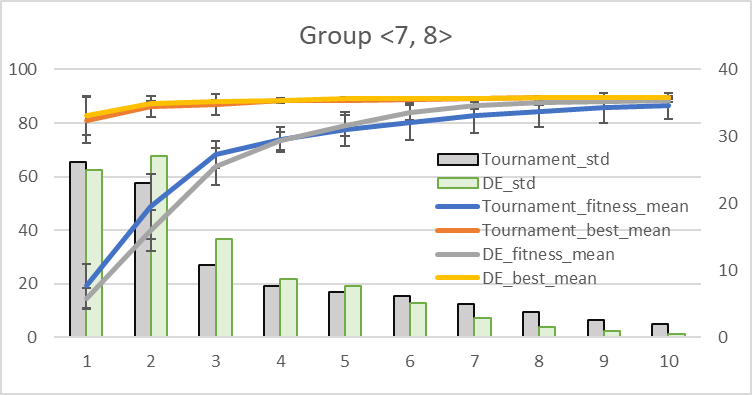
\includegraphics[width=\textwidth]{fig/g78_2.png}
        \caption{Enemy group <7,8>}
        \label{fig:gain_1}
    \end{subfigure}
    \hfill
    \begin{subfigure}[htbp]{0.55\textwidth}
        \centering
        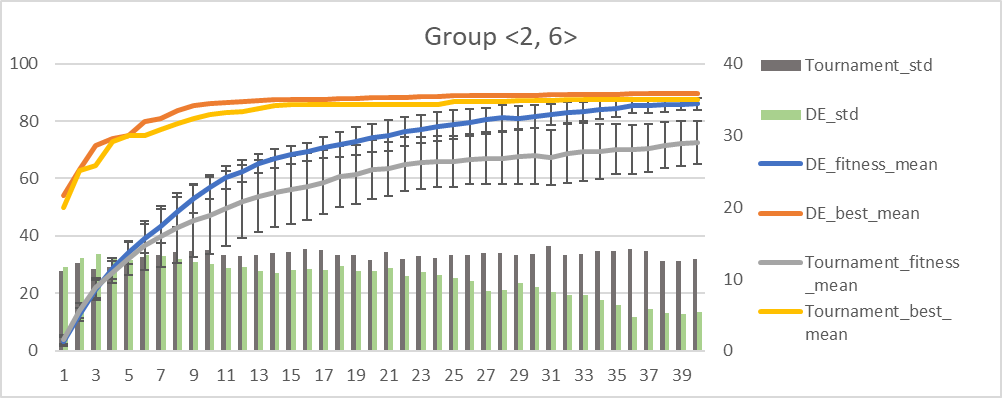
\includegraphics[width=\textwidth]{fig/g26_2.png}
        \caption{Enemy group <2,6>}
        \label{fig:gain_2}
    \end{subfigure}
    \caption {Fitness of 2 EAs over multiple enemies}
    \label{fig:gain}
\end{figure*}

\subsection{Comparison of Two EA Methods and Expection on Result}
As illustrated in section \ref{sec:psel}, both EA methods are designed to balance diversity and convergence speed but may behave differently. The key differences between the two methods lie in parent selection and mutation strategies. Both employ random two-point crossover.

For parent selection, both EAs implement tournament selection for at least one of the parents, while both parents are selected by tournament in EA1, EA2 ensures the participation of all individuals in the population in the evolutionary process. Thus theoretically, EA1 will introduce higher selection pressure on parents than EA2.

Apart from the selection pressure, the two EAs have different mutation step lengths, while EA 1 constrains the variation distance, namely the bounds on search space, with a fixed mutation rate set at 0.2, the mutation rates of EA 2 are different between the generations.

As mentioned in section \ref{sec:improve}, In EA2, the mutation process comprises two components: the differential vector and the noise vector. The mutation vectors which are dependent on the difference between two randomly selected individuals theoretically result in a high mutation rate initially when individuals are diverse, which can lead to a rapid decrease in the standard deviation of the whole population. However, as there is less selection pressure compared to EA1, it is not guaranteed all individuals would converge to the best fitness. While in EA1, there will be more chance that the recombination happens on above-average parents.

%(Results and discussion: discuss the differences between the results of your EAs; do they outperform each other? Comment on a possible explanation for that; Discuss the differences between your results and the results of the baseline paper; are they better/equal/worse? Comment on a possible explanation for that.)


\subsection{Average/std performances in 2 EAs}
As depicted in Figure \ref{fig:gain}, it's evident that the two Evolutionary Algorithms (EAs) exhibit similar convergence speeds within the same experimental context, with both demonstrating more rapid progress in the <7,8> enemy group.

Irrespective of the training set, an interesting pattern emerges. In the initial stages, EA1 displays a more rapid convergence compared to EA2. However, as the training progresses, EA2 surpasses EA1, ultimately achieving a higher average fitness in the later stages. In general, EA2 exhibits faster overall convergence, thus substantiating the validity of the first hypothesis.

This observation suggests that in the initial stages, EA2, due to higher selection pressure on parents, is more likely to generate offspring from the best or better-fitted individuals. Nevertheless, as mutations are randomly generated with fixed step lengths in EA1, the new generation retains a degree of diversity. In contrast, EA2, with its differential vector mechanism, facilitates rapid clustering within the population, even though it doesn't guarantee that higher-fitness individuals are more likely to mate. However, after several generations of survivor selection, clusters with lower fitness levels tend to be eliminated, leaving the remaining individuals with a higher likelihood of converging toward the best fitness.

The standard deviation of fitness, as illustrated in Figure \ref{fig:gain_2}, further corroborates the observation that EA1 sustains a higher level of diversity throughout the evolution. This diversity can be indicative of a more extensive exploration of the search space. However, it comes at the cost of a slower increase in the mean fitness over time.

Upon comparing the two experiments, it becomes evident that when confronted with a challenging training environment, such as the enemy pair <2,6>, the discrepancy in convergence speed becomes more significant. This observation suggests that, in scenarios where time efficiency is a crucial factor, opting for EA2 could be a more favorable choice.
%This fact might imply that, in the initial stage, as EA 2 undergoes higher selection pressure on parents, the new generation has a higher chance of being the offspring of the best or the better-fitted individuals. However, since the mutations are randomly generated and the step length is fixed in EA1, the new generation would maintain diversity. While in EA2, the population tends to cluster rapidly as the differential vector helps to minimize their distance (comparing to EA 1), but since all the individuals participated in the mate, It is not guaranteed that higher-fitted individuals mate more. However, after several generations of survivor selection, the clusters with bad fitness be dropped, and the remaining individuals would be more likely to converge to the best fitness.

%Comparing the two experiments, when facing a complicated training environment, such as enemy pair <2,6>, the converge speeddifference would be more significant.

%With the basic theory of evolutionary computing, we apply the algorithm of crossover with two different operators: Random crossover and crossover with tournament. Figure 1 shows the result of the average/standard deviation of the fitness over the 8 enemies. In general, the fitness of all the eight enemies has a trend of increasing and converge to a fixed value. The mean of the fitness start at a relatively low fitness score at early generations while the maximum fitness score starts higher and finally converge to its stable point and there is no obvious difference between the values of best fitness in 2 EAs and they show similar best fitness number in most cases. 

%We then pick the result of 1, 2, 6 for analysis. By comparison with Figure 1 , it is noticeable that EA2 algorithm works faster to reach the best fitness. EA2 model shows the steeper rise and uses less generations to fit into the best solution. This implies the that tournament of the crossover between parents would influence the converge rate. When coming across the enemy 1, these 2 EAs both perform the relatively harder evolutionary process, with the most number of generations in 8 enemies. However, it could be observed that EA1 experienced a longer generations of evolution than EA2. In the experiment with enemy 2, it could be observed that the maximum fitness starts near the best while the mean of the fitness experienced a very steep converge to its limit in a very small numbers of generation. The standard deviation shows its confidence interval is relatively small. It implies that this enemy is stable and easier to predict than other enemies. When encountering enemy 6, there is a clear advantage of EA2 that the status becomes stable at generation 40 while in EA1, it takes approximately 80 generation to converge to stable point.

\subsection{Comparisons of best solutions in 2 EAs}
\begin{figure}[htbp]
    \centering
    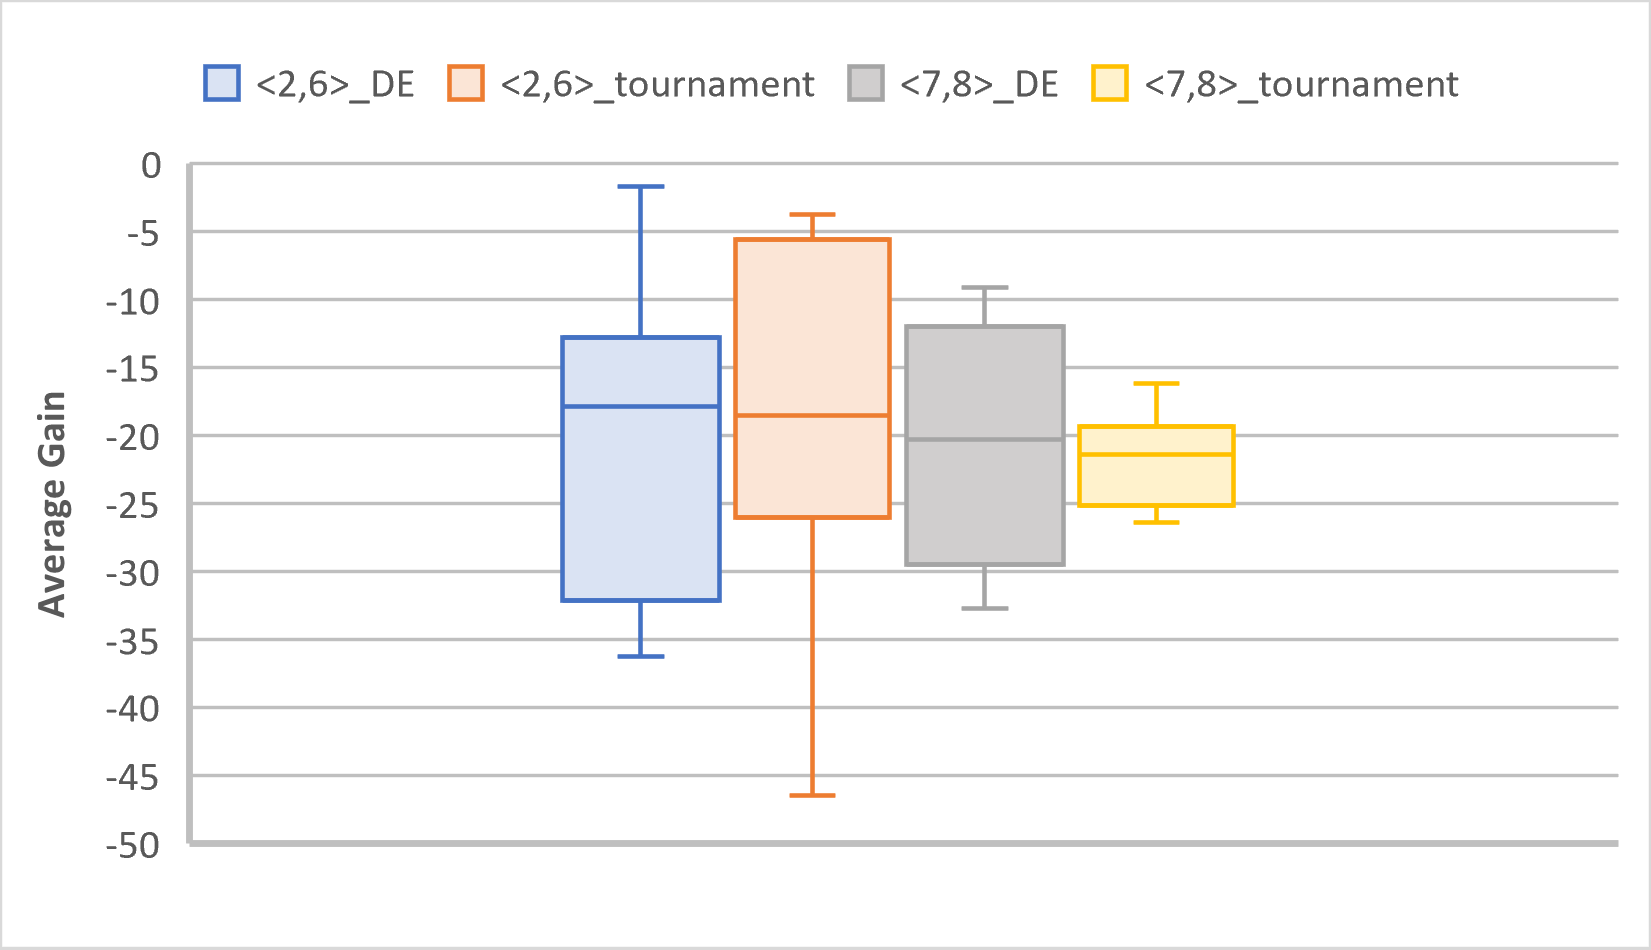
\includegraphics[width=0.9\columnwidth]{fig/gains.png}    
    \caption {Fitness of 2 EAs over multiple enemies}
    \label{fig:test}
\end{figure}
Figure \ref{fig:test} illustrates the individual gains achieved by both EAs across eight different enemy scenarios, each subjected to ten rounds of experimentation. In EA1, there appears to be a higher probability that when the population rapidly converges, particularly evident in the <7,8> group, the ultimate best solution may lose diversity. Conversely, in EA2, the lower selection pressure in the initial stage allows for more extensive exploration within each solution.

In the <2,6> enemy pair scenario, this problem is less pronounced. Since the mutation step remains fixed, the population can explore a broader search space. Consequently, EA1, which exhibits slower progress, may uncover superior solutions through deeper exploration. This outcome, being probabilistic, conditionally supports the hypothesis 2.

Upon comparing the two EA approaches, EA2 achieves a higher best score of gain, while another solution from EA1 manages to defeat more enemies, totaling 5. %A detailed summary of the outcomes and comparisons with the baseline algorithm can be found in Table.

\section{Conclusion}
In this report, we have presented a thorough introduction to the design and underlying motivation of the two Evolutionary Algorithms (EAs). Through a comparative analysis of their performance in two distinct experiments, we have unveiled their strengths, potential drawbacks, and provided insights into when each EA is most suitable for a given scenario.
%\newpage

\begin{comment}
\begin{thebibliography}{}
\bibitem{Paper}
Agoston E. Eiben \& Jim Smith (2016) \emph{From evolutionary computation
to the evolution of things}, doi:10.1038/nature14544.

\bibitem{book}
Agoston E. Eiben \& Jim Smith (2015) \emph{Introduction to Evolutionary Computing: Second Edition}, Springer

\bibitem{Paper}
K. Araujo \& F. Franca (2015) \emph{An electronic-game framework for evaluating co-evolutionary algorithms}, 

$https://doi.org/10.48550/arXiv.1604.00644$

\bibitem{Paper}
K. Araujo \& F. Franca (2016) \emph{Evolving a Generalized Strategy for an Action-Platformer Video Game Framework}, 

$https://doi.org/10.48550/arXiv.1604.00644$

\bibitem{Paper}
J. Koza (2009) \emph{Human-competitive results produced by genetic
programming},

doi 10.1007/s10710-010-9112-3


\end{thebibliography}
\end{comment}